% Supplementary material for "From Trajectories to Evidence: Auditing
% Observation Loss and Identifiability in Computer-Use Agent Evaluation"
% (AAMAS 2027 main-track submission). Submitted as a separate zip per the
% AAMAS 2027 call for papers ("supplementary material" is optional and
% reviewed at reviewers' discretion; it does not count against the 8-page
% main-track limit). Split out of draft/main.tex 2026-09-14.
% Compile: pdflatex supplementary && bibtex supplementary && pdflatex supplementary && pdflatex supplementary
\documentclass[sigconf,anonymous]{aamas}

\usepackage{amsmath,amssymb}
\usepackage{enumitem}
\usepackage{array}

\graphicspath{{../../../out/stage4_counterfactual_analysis_final/}}

\hypersetup{colorlinks=true,linkcolor=black,citecolor=black,urlcolor=black}

\newcommand{\task}[1]{\texttt{#1}}
\newcommand{\A}{\mathcal{A}}
\newcommand{\Acap}{\mathcal{A}^{\cap}}
\newcommand{\STS}{\mathrm{STS}}
\newcommand{\Just}{\mathrm{Justifiable}}

%%% AAMAS-2027 copyright block (do not change!)
\makeatletter
\gdef\@copyrightpermission{
  \begin{minipage}{0.2\columnwidth}
   \href{https://creativecommons.org/licenses/by/4.0/}{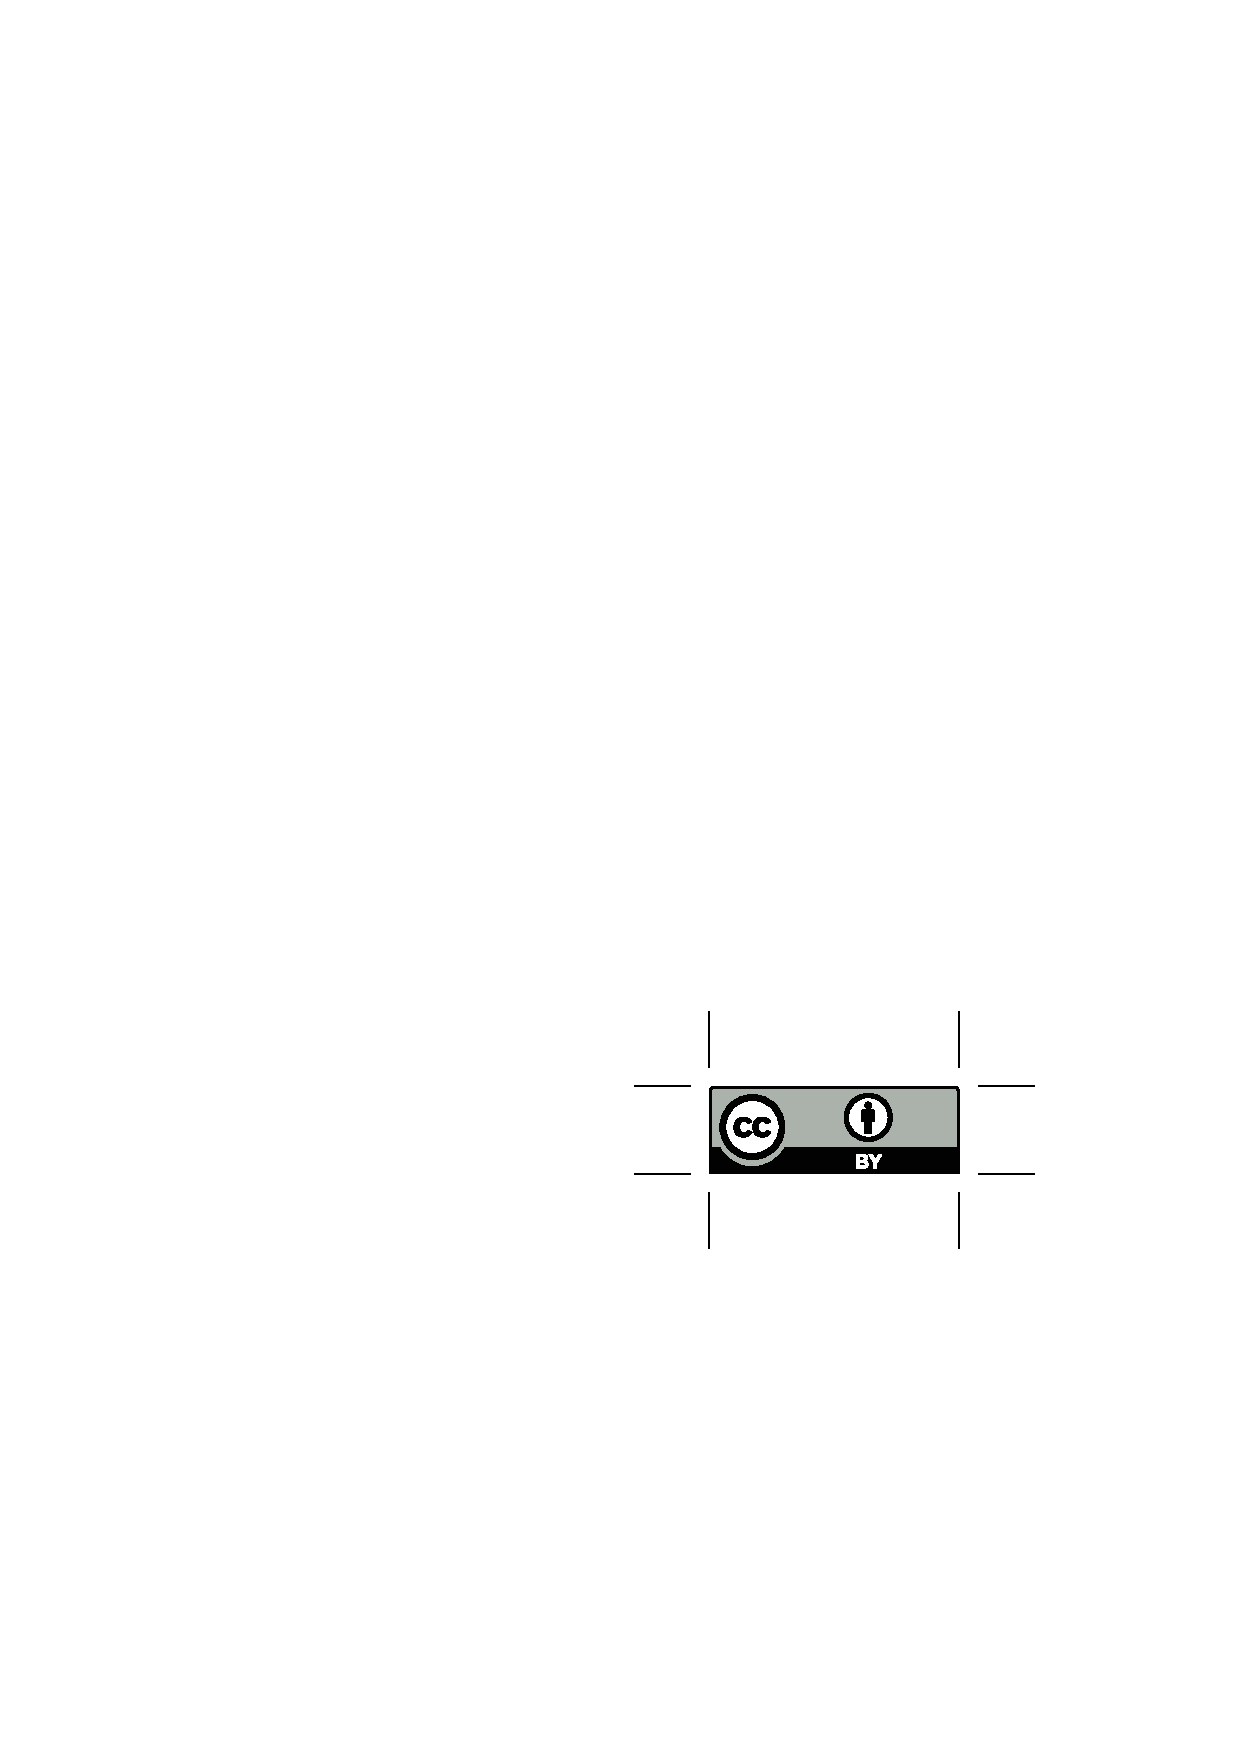
\includegraphics[width=0.90\textwidth]{by}}
  \end{minipage}\hfill
  \begin{minipage}{0.8\columnwidth}
   \href{https://creativecommons.org/licenses/by/4.0/}{This work is licensed under a Creative Commons Attribution International 4.0 License.}
  \end{minipage}
  \vspace{5pt}
}
\makeatother

\setcopyright{ifaamas}
\acmConference[AAMAS 2027]{Proc.\@ of the 26th International Conference
on Autonomous Agents and Multiagent Systems (AAMAS 2027)}{3--7 May 2027}{Hanoi, Vietnam}{M.~Baldoni, F.~Fang, W.~Yeoh, N.~Yorke-Smith (eds.)}
\copyrightyear{2027}
\acmYear{2027}
\acmDOI{}
\acmISBN{}
% TODO(vinh): fill in the OpenReview submission id once assigned (same id as main.tex).
\acmSubmissionID{}
\submissionType{Research Paper Track}

\title{From Trajectories to Evidence: Supplementary Material}

% TODO(vinh): same placeholder convention as draft/main.tex -- authors unset,
% anonymous mode hides this from the typeset PDF regardless.
\author{Anonymous Author(s)}
\affiliation{%
  \institution{Institution withheld for review}
  \country{}}
\email{}

\begin{abstract}
This document is supplementary material for the AAMAS 2027 main-track
submission ``From Trajectories to Evidence: Auditing Observation Loss and
Identifiability in Computer-Use Agent Evaluation.''
Per the AAMAS 2027 call for papers, supplementary material is optional,
does not count against the 8-page main-track limit, and is consulted by
reviewers at their discretion; it is not a substitute for, or an
extended/corrected version of, the submitted paper.
Appendices~A--E below were Appendices~A--E of the main paper before this
split; all labels, table/figure numbers, and content are unchanged.
\end{abstract}

\begin{document}
\maketitle

\section{Study 1 details}
\label{app:s1}

Study~1 is an existence / dissociation demonstration, not a prevalence estimate.
The frozen schedule executed 46 of 50 intended cells (92 legs).
35 legs are execution failures; 24 pairs are valid.
Primary lanes are reported separately (Table~\ref{tab:s1}).
A size ablation and an exploratory Flash lane exist and are not pooled.
We do not headline a pooled invariance rate.

\begin{table}[H]
\centering
\caption{Study~1 primary lanes (existence sample). Invariance is Type~A over tracking-valid pairs. Intervals are Clopper--Pearson 95\% and are wide. Source: Stage-4 snapshot \texttt{b7b4203}.}
\label{tab:s1}
\small
\begin{tabular}{lrrrrr}
\toprule
Lane & Valid & Track-valid & Type~A & Sens.\ & Type~B \\
\midrule
Claude          & 9 & 7 & 6 & 1 & 2 \\
GPT-5.5         & 8 & 7 & 3 & 4 & 1 \\
Qwen3.5-35B-A3B & 1 & 1 & 1 & 0 & 0 \\
\bottomrule
\end{tabular}
\end{table}

Claude: invariance $6/7=0.857$ ($[0.421,0.996]$).
GPT-5.5: $3/7=0.429$ ($[0.099,0.816]$).
Qwen3.5-35B-A3B: one valid pair, Type~A ($[0.025,1.000]$).
Paired world interventions follow a counterfactual design~\citep{pearl2009causality}; they are a method for this dissociation, not the paper's main contribution.

\begin{figure}[H]
\centering

\includegraphics[width=0.98\columnwidth]{score_pairs_primary.png}
\caption{Study~1 primary lanes: paired base vs.\ counterfactual scores on valid pairs. Ablation and exploratory lanes are not pooled into Table~\ref{tab:s1}.}
\label{fig:s1pairs}
\end{figure}

\section{Study 2 details}
\label{app:s2}

Locked heading: evaluation and selection can change the evidential basis of a reliability comparison.
It is not a claim that the evaluator changes the truth.

Three agents each ran a pre-registered schedule of 57 legs: GPT-5.5, Qwen3.8-Flash, and Claude Opus~4.6 (Table~\ref{tab:coverage}).
The inclusion threshold $n_{\min}=3$ valid pairs to be ranked, and the rule that fewer than three ranked agents means the confirmatory selection test is \emph{not evaluated}, were committed before any outcome existed.

\begin{table}[H]
\centering
\caption{Coverage under the frozen instrument. A valid pair requires both legs to terminate. Claude's mean $S^{0}$ is a single pair. Freeze: tag \texttt{paper2-frozen} on commit \texttt{39cc662}. Not a ranking of 57 tasks.}
\label{tab:coverage}
\small
\begin{tabular}{lrrrrr}
\toprule
Agent & DONE/57 & $|\A|$ & mean $S^{0}$ & mean $\STS$ \\
\midrule
GPT-5.5         & 32 & 9 & 69.3 & 0.130 \\
Qwen3.8-Flash   & 29 & 8 & 95.8 & 0.229 \\
Claude Opus 4.6 &  4 & 1 & 100  & 0 \\
\bottomrule
\end{tabular}
\end{table}

Claude terminated on four legs across three tasks, so $|\A|=1$.
The ranked roster is two agents, which is fewer than three, and the confirmatory selection test is therefore not evaluated.

On a four-task common support, labelled exploratory, a paired bootstrap (seed $20260904$, $B=5000$) gives Flash-minus-GPT $\Delta S^{0}=+46.5$ (95\% CI $[21.0,72.0]$) and $\Delta\STS=-0.042$ ($[-0.125,0.000]$).
The reversal is strict on one task (\task{retrieval-f009}) and tied on three.
Removing that task makes the $\STS$ comparison a tie.
We make no claim about the prevalence of ranking instability.

Conditioning on termination also changes what the score can see.
Excluded cells score lower on average (mean $S$ off $\A$: $46.4$, $44.9$, $26.1$ against $69.3$, $95.8$, $100$ on $\A$).
What survives that average is sharp: 2, 2, and 1 excluded cells scored $\ge 90$ with no canonical \texttt{DONE}.
A completion-conditioned protocol cannot express rubric-visible progress without closure.

\section{Study 3 secondary diagnostics}
\label{app:s3}

Table~\ref{tab:repairs-full} is the full layer-repair diagnostic (134 rows).
R-SCOPE converts 14 of 20 already-correct rows into something else.
R-CHAN destroys 7 MATCH rows.
R-CMP is bit-identical to FROZEN.

\begin{table}[H]
\centering
\caption{Layer repairs as diagnostic interventions, 134 rows. Sensitivity is over 59 R1-positive rows.}
\label{tab:repairs-full}
\footnotesize
\setlength{\tabcolsep}{4pt}
\begin{tabular}{lrrrr}
\toprule
Config & Sens./59 & Abst./134 & M4/reported & MATCH dest./20 \\
\midrule
FROZEN  & 20 &  89 & 25/45 &  0 \\
R-AGG   & 28 &  63 & 43/71 &  0 \\
R-SCOPE & 13 &  56 & 65/78 & 14 \\
R-CMP   & 20 &  89 & 25/45 &  0 \\
R-CHAN  & 15 & 104 & 15/30 &  7 \\
ALL     & 10 &  79 & 45/55 & 16 \\
\bottomrule
\end{tabular}
\end{table}

On the same four-task support as Study~2, R-CHAN inverts the sign of Flash-minus-GPT $\Delta\STS$ ($-0.0417\to +0.1667$) because GPT collapses ($0.250\to 0.042$) while Flash is unchanged.
The effective number of independent task-clusters for the frozen $\Delta\STS$ is one.
This is an existence demonstration, not a claim that rankings are unstable in general.

A locked, corpus-independent reconstruction rule recovers 9 of 30 hand-written label components (G2 FAIL).
Groundedness against the task definition is 100\% (G1).
A pre-specified comparative-scale gate required 20 independent task clusters; 16 of 28 candidates survived a frozen feasibility probe, so that experiment was not opened.

\section{M1a rows joined to locked scores}
\label{app:m1a-join}

Post-hoc join of the 13 locked M1a rows to Study~2 $S$, $Y$, and (where present) earlier-trajectory text.
Gold in the final answer and in \texttt{found} is definitional for M1a.
$S$ is the screenshot-rubric score on that leg; $Y$ is pair-level binary tracking.
Three rows have no locked per-leg $S$ and are left unknown.
Earlier text means the gold string occurs in \texttt{action}/\texttt{response} fields of \texttt{traj.jsonl} lines before the last line; PNG files were not read.
Denominator: 13 M1a rows, not 171 legs.
Source: \texttt{paper/evaluation\_measurement\_gap/experiment\_m1a\_location/}.

\begin{table*}[t]
\centering
\caption{Thirteen M1a rows. $S{=}100$ counts use the 10 joinable rows only.}
\label{tab:m1a-join}
\small
\setlength{\tabcolsep}{5pt}
\begin{tabular}{lllcrrcc}
\toprule
Lane & Task & Leg & Component & $S$ & $Y$ & DONE & Earlier text \\
\midrule
Flash & \task{counterfactual-f010} & G0 & liquid\_cash & 100 & 0 & yes & yes \\
Flash & \task{counterfactual-f013} & G0 & batbucks\_dividends & 100 & 0 & yes & yes \\
Flash & \task{counterfactual-f013} & G0 & gringotts\_savings & 100 & 0 & yes & no \\
Flash & \task{counterfactual-f013} & G1 & gringotts\_savings & 100 & 0 & yes & yes \\
Flash & \task{retrieval-f009} & G1 & nyc\_flight\_confirmation & 100 & 0 & yes & yes \\
Flash & \task{retrieval-f010} & G1 & host\_name & 100 & 0 & yes & yes \\
GPT-5.5 & \task{aggregation-f020} & G0 & batbucks\_cash & 83 & 0 & yes & no \\
GPT-5.5 & \task{retrieval-f009} & G0 & nyc\_hotel\_confirmation & 40 & 0 & yes & no \\
GPT-5.5 & \task{retrieval-f009} & G1 & nyc\_flight\_confirmation & 40 & 0 & yes & no \\
Flash & \task{counterfactual-f005} & G1 & gme\_shares & 100 & --- & no & yes \\
Claude & \task{counterfactual-f005} & G0 & gme\_avg\_cost & --- & --- & --- & yes \\
Claude & \task{counterfactual-f005} & G0 & gme\_shares & --- & --- & --- & yes \\
Flash & \task{aggregation-f020} & G1 & batbucks\_cash & --- & --- & --- & no \\
\bottomrule
\end{tabular}
\end{table*}

\section{Admitted string/URL FAIL composition}
\label{app:patha}

Supporting check only (ledger A-FAIL, A-AB).
Not an AgentRewardBench-wide audit, not an admission-set prevalence, and not a rate of unjustified FAIL.
AssistantBench is I-emptiness only and is not pooled into 126/299.
HIT/MISS against gold is not reported here.

\begin{table*}[t]
\centering
\caption{Released oracle FAIL on ELIGIBLE episodes, split by whether locked last-answer/last-URL $I$ is empty. Determining FAIL means a candidate was present and did not match (WA/VWA) or, for AssistantBench, that a last \texttt{send\_msg\_to\_user} existed (gold not opened).}
\label{tab:patha-fail}
\small
\begin{tabular}{@{}lrrr@{}}
\toprule
Slice & Empty $I$ & Candidate present & Released FAIL \\
\midrule
WebArena string/URL & 52 & 93 & 145 \\
VisualWebArena string/URL & 74 & 80 & 154 \\
WA$+$VWA (licensed) & 126 & 173 & 299 \\
AssistantBench (emptiness only) & 62 & --- & 115 \\
\bottomrule
\end{tabular}
\end{table*}

As a sensitivity join only (not correspondence gold): among the 299 released FAIL, AgentRewardBench human \texttt{trajectory\_success} is Successful on 4/126 empty-$I$ trajectories and on 50/173 mismatch trajectories (318 of 366 ELIGIBLE WA/VWA episodes have a single annotator).
Empty-$I$ FAIL is not the hidden-success pocket; human-labeled success, when it occurs among FAIL, concentrates on candidate-then-mismatch---the setting already studied as rule-based under-reporting~\citep{lu2025agentrewardbench,dong2026misscore}.
The two FAIL kinds are therefore not exchangeable even against human labels.
This is not a rate of unjustified FAIL.


\bibliographystyle{ACM-Reference-Format}
\bibliography{refs}

\end{document}
